\documentclass[10pt]{beamer}

\newcommand{\lectnum}{L08}
\newcommand{\lecttitle}{Kernels and Support Vector Machines}

\usepackage{amsmath, amssymb, graphicx}
\usepackage[]{algorithm2e}
\usepackage{pdfpages}
\usepackage[british]{babel}

\hypersetup{colorlinks,linkcolor=,urlcolor=blue}
\newenvironment{titledslide}[1]{\begin{frame}\frametitle{#1}}{\end{frame}}

\mode<presentation>{\setbeamercovered{transparent}}

\setbeamertemplate{sidebar right}{}
\setbeamertemplate{footline}{%
\hfill\usebeamertemplate***{navigation symbols}
\hspace{0.4cm}\lectnum: \insertframenumber{}/\inserttotalframenumber \hspace*{0.4cm}}

\author{James Cussens}

\title{COMS30035, Machine learning:\\ \vspace{5pt} \lecttitle}

\institute{School of Computer Science\\University of Bristol}

\begin{document}
%%%%%%%%%%%%%%%%%%%%%%%%%%%%%%%%%%%%%%%%%%%%%%%%%%%%%%%%%%%%%%%%%%%%%%

\begin{frame}
  \titlepage
\end{frame}

%%%%%%%%%%%%%%%%%%%%%%%%%%%%%%%%%%%%%%%%%%%%%%%%%%%%%%%%%%%%%%%%%%%%%%


\newcommand{\params}{\ensuremath{\mathbf{w}}}
\newcommand{\dualparams}{\ensuremath{\mathbf{a}}}
\newcommand{\designm}{\ensuremath{{\bm \Phi}}}
\newcommand{\xvec}{\ensuremath{\mathbf{x}}}
\newcommand{\feat}{\ensuremath{\phi}}
\newcommand{\gram}{\ensuremath{\mathbf{K}}}
\newcommand{\xvecn}{\ensuremath{\mathbf{x}_{n}}}

%%%%%%%%%%%%%%%%%%%%%%%%%%%%%%%%%%%%%%%%%%%%%%%%%%%%%%%%%%%%%%%%%%%%%%
\begin{titledslide}{Extracting features}

  \begin{itemize}
  \item Let's have a look at \cite[p.370]{pml1Book}
  \end{itemize}
  
\end{titledslide}
%%%%%%%%%%%%%%%%%%%%%%%%%%%%%%%%%%%%%%%%%%%%%%%%%%%%%%%%%%%%%%%%%%%%%%
\begin{titledslide}{tldr version}

  Suppose we're doing classification where each training data point
  is $(\xvec,y)$.
  
  \begin{description}
  \item[Standard approach] Choose a function $\feat$. Map each raw
    data vector $\xvec$ into a feature vector $\feat(\xvec)$. Learn
    parameters using the feature vectors and class labels. When making a
    prediction for a test data vector $\xvec'$ first encode as
    $\feat(\xvec')$ and use learned model to make prediction.
  \item[Kernel approach] Choose a kernel function $k$ which
    (intuitively) measures similarity between raw data vectors
    $k(\xvec_{m},\xvec_{n})$. Learn parameters using the
    $k(\xvec_{m},\xvec_{n})$ values and class labels. When making a
    prediction for a test data vector $\xvec'$ use learned parameters
    and values of $k(\xvec_{n},\xvec')$ to make a prediction.
  \end{description}

  
\end{titledslide}


% \begin{frame}[fragile]
% \frametitle{Agenda}
% \begin{itemize}
% \item Dual representations
% \item Kernel functions
% \item The `kernel trick'
% \item The reading associated with this lecture is
%   \cite[p.291--294]{bishop06:_patter_recog_machin_learn}.
% \end{itemize}
% \end{frame}


\begin{frame}[fragile]
\frametitle{(Regularised) Linear regression revisited}
Suppose we are doing (regularised) linear regression by minimising
regularised sum of squared error:
\begin{equation}
  \label{eq:lr}
  J(\params) = \frac{1}{2}
  \sum_{n=1}^{N}\left(\params^{\top}\feat(\xvec) - t_{n}\right)^{2} + \frac{\lambda}{2}\params^{\top}\params
\end{equation}
where
\begin{enumerate}
\item \params{} is the $M$-dimensional parameter vector to be learned
  from the data (which includes a component for the intercept)
\item \xvec{} is some datapoint, and
\item $\feat(\xvec)$ is the $M$-dimensional feature vector which
  \xvec{} gets mapped to by the \emph{basis functions}
  \cite[\S3.1]{bishop06:_patter_recog_machin_learn}.
\item $\frac{\lambda}{2}\params^{\top}\params$ is the regularisation
  term which pushes parameters which are not helping much to fit the
  data towards zero.
\end{enumerate}
\end{frame}

\begin{frame}[fragile]
\frametitle{Dual representations}
\begin{itemize}
\item Let $N$ be the size of the data. Let $\designm$ be the
  \emph{design matrix} whose $n$th row is just the feature vector for
  the $n$th datapoint (so it is basically `the data'). It turns out that
  we can write the minimising value of $\params$ in terms of an $N$-dimensional parameter vector
  \dualparams{} as follows:
\end{itemize}
\begin{equation}
  \label{eq:dualone}
  \params = \designm^{T} \dualparams
\end{equation}
so that
\begin{equation}
  \label{eq:dual}
  y(\xvec) = \params^{T}\feat(\xvec) = \dualparams^{T}\designm\feat(\xvec)
\end{equation}

In this case, the \emph{dual parameters} $a_n$ are the
($\lambda$-adjusted) \emph{residuals}:
\begin{equation}
  \label{eq:duala}
  a_{n} = -\frac{1}{\lambda}\left( \params^{T}\feat(\xvecn) - t_{n}\right)
\end{equation}


\begin{itemize}
\item Using $\dualparams$ is known as a \emph{dual representation}.
\item So we have replaced an $M$-dimensional parameter vector with an
  $N$-dimensional one and moreover, to make a prediction for a new
  datapoint we have to use the entire training set (i.e.\ \designm)
\item On the face of it this does not seem such a great idea, (unless perhaps $M$ is much bigger than $N$).
\end{itemize}
\end{frame}

\begin{frame}[fragile]
\frametitle{Kernel functions are scalar products in feature space}


Suppose $\xvec$ is some test datapoint. Let's have a look at $\designm\feat(\xvec)$.
Suppose, for example, that we had 3 datapoints $\xvec_{1}$, $\xvec_{2}$ and $\xvec_{3}$ and 2 features so

\begin{equation}
  \label{eq:expdotp}
  \designm\feat(\xvec) =
  \begin{pmatrix}
    \phi_{1}(\xvec_{1}) & \phi_{2}(\xvec_{1})  \\
    \phi_{1}(\xvec_{2}) & \phi_{2}(\xvec_{2})  \\
    \phi_{1}(\xvec_{3}) & \phi_{2}(\xvec_{3})  
  \end{pmatrix}
  \begin{pmatrix}
  \phi_{1}(\xvec) \\ \phi_{2}(\xvec) 
\end{pmatrix}
=
\begin{pmatrix}
  \phi(\xvec_{1})^{T}\phi(\xvec)  \\
  \phi(\xvec_{2})^{T}\phi(\xvec)  \\
  \phi(\xvec_{3})^{T}\phi(\xvec)  \\
\end{pmatrix}
\end{equation}

If we define a \emph{kernel function}
\begin{equation}
  \label{eq:kerneldef}
  k(\xvec,\xvec') =   \phi(\xvec)^{T}\phi(\xvec')
\end{equation}

then we can write:
\begin{equation}
  \label{eq:kerntwo}
    \designm\feat(\xvec) = \begin{pmatrix}
      k(\xvec_{1},\xvec)  \\
      k(\xvec_{2},\xvec)  \\
      k(\xvec_{3},\xvec)  \\
      \end{pmatrix}
\end{equation}

\end{frame}

\begin{frame}[fragile]
  \frametitle{The kernel trick}

  So the prediction for datapoint \xvec{} in our example is:
  \begin{equation}
    \label{eq:predxvec}
    \dualparams^{T}\designm\feat(\xvec) = \dualparams^{T} \begin{pmatrix}
      k(\xvec_{1},\xvec)  \\
      k(\xvec_{2},\xvec)  \\
      k(\xvec_{3},\xvec)  \\
      \end{pmatrix}
  \end{equation}
  
  \begin{itemize}
  \item The key point is that \textbf{we just need the kernel function} to make the prediction.
  \item The `kernel trick' is to evaluate the kernel function values, e.g.\       $k(\xvec_{1},\xvec)$ without first computing $\feat(\xvec_{1})$ and $\feat(\xvec)$ and then computing their scalar product.
  \item This allows us to use very high-dimensional (even infinite dimensional!) feature spaces since features are never directly computed.
  \end{itemize}
\end{frame}

\begin{frame}[fragile]
  \frametitle{Kernel functions and similarity}

  \begin{itemize}
  \item A kernel function represents the degree of `similarity' between its two arguments (so kernel functions are always symmetric).
  \item A high kernel value represents a high degree of similarity.
  \item Returning to our example, the prediction for $\xvec$ is:
  \end{itemize}
  \begin{equation}
    \label{eq:foo}
    y(\xvec) = \dualparams^{T} \begin{pmatrix}
      k(\xvec_{1},\xvec)  \\
      k(\xvec_{2},\xvec)  \\
      k(\xvec_{3},\xvec)  \\
    \end{pmatrix}
    = a_{1}k(\xvec_{1},\xvec)  + a_{2}k(\xvec_{2},\xvec)  + a_{3}k(\xvec_{3},\xvec) 
  \end{equation}
  \begin{itemize}
  \item So the prediction for $\xvec$ is a linear function of the `similarities' between \xvec{} and each element of the training data.
  \item So unlike, say, linear regression it looks like we have to keep the entire training set around to make predictions. \pause
  \item But in fact we only need those $\xvec_{i}$ where $a_{i} \neq 0$. (See later on \emph{support vector machines}.)
  \end{itemize}

\end{frame}

\begin{frame}[fragile]
\frametitle{Learning with kernels}

\begin{itemize}
\item So far we have focused on making predictions using a learned value of the dual parameter vector \dualparams.
\item If we needed to compute feature values $\feat(\xvec)$ to learn \dualparams, then the advantage of using kernels would disappear.
\item But the good news is that (for many models) we can learn \dualparams{} just using kernels.
\item So both learning and predicting just require evaluating kernel functions.
\end{itemize}
\end{frame}

\begin{frame}[fragile]
\frametitle{The Gram matrix}

\begin{itemize}
\item The \emph{Gram matrix} $\gram$ is defined to be $\designm \designm^{T}$.
\item So $K_{nm} = \phi(\xvec_{n})^{T}\phi(\xvec_{m}) =
  k(\xvec_{n},\xvec_{m})$ is the `similarity' between the $n$th and
  $m$th datapoint.
\item Given data (the $\xvec_{n}$) and a particular choice of kernel
  $k$, we can compute the Gram matrix $\gram$.
\item $\gram$ is what we need for learning.
\item Note that $\gram$ is symmetric.
\end{itemize}


\end{frame}

\begin{frame}[fragile]
\frametitle{Learning with kernels example (1)}

\begin{itemize}
\item Suppose we want to add a quadratic regulariser (aka \emph{weight decay}) term when minimising the squared error on the training set \params{} \cite[\S3.1.4]{bishop06:_patter_recog_machin_learn}.
\item Then, if we were not using kernels, our goal \cite[(6.2)]{bishop06:_patter_recog_machin_learn} is to minimise $J(\params)$ where: 
\end{itemize}
\begin{equation}
  \label{eq:l2}
  J(\params) = \frac{1}{2} \sum_{n=1}^{N} \left\{ \params^{T}\feat(\xvec_{n}) - t_{n} \right\}^{2} + \frac{\lambda}{2} \params^{T}\params
\end{equation}
\begin{itemize}
\item $N$ is the number of training datapoints, $\lambda$ is the regularisation parameter and $t_n$ is the observed target value of the $n$th training datapoint.
\end{itemize}
\end{frame}

\begin{frame}[fragile]
\frametitle{Learning with kernels example (2)}

\begin{itemize}
\item Let $\mathbf{t} = (t_{1}, \dots, t_{N})^{T}$ and let $\mathbf{I}_{N}$ be the $N \times N$ identity matrix then it turns out that setting:
\end{itemize}

\begin{equation}
  \label{eq:ahat}
  \dualparams = (\gram + \lambda \mathbf{I}_{N})^{-1}\mathbf{t}
\end{equation}

\begin{itemize}
\item is equivalent to minimising $J(\params)$ (see \cite[\S6.1]{bishop06:_patter_recog_machin_learn} for the necessary algebra).
\item The key point is that the dual parameters can be learned just using kernels and without computing any feature values.
\end{itemize}

\end{frame}


% \begin{frame}[fragile]
% \frametitle{Agenda}
% \begin{itemize}
% \item Max margin classification
% \item Support vector machines
% \end{itemize}
% \end{frame}


\begin{frame}
\frametitle{Recap}
\begin{itemize}
\item Earlier we saw an example of:
  \begin{enumerate}
  \item learning: $\dualparams = (\gram + \lambda \mathbf{I}_{N})^{-1}\mathbf{t}$
  \item and computing predicted values:  $y(\xvec) = a_{1}k(\xvec_{1},\xvec)  + a_{2}k(\xvec_{2},\xvec)  + a_{3}k(\xvec_{3},\xvec)$
  \end{enumerate}
where both were done using only a kernels
\item But for learning we needed to compute the kernel value for every pair of training datapoints, and for prediction we needed the entire training set.
\item \emph{Support vector machines} are a kernel-based method for classification which avoids this excessive computation.
\item We still also need to address the question of which kernel function to use, more on this later \dots
\end{itemize}
\end{frame}
%%%%%%%%%%%%%%%%%%%%%%%%%%%%%%%%%%%%%%%%%%%%%%%%%%%%%%%%%%%%%%%%%%%%%% 
\begin{frame}
\frametitle{Linear classification}
Consider a simple linear model for two class classification:
\begin{equation}
  \label{eq:lindiscrim}
    y(\xvec) = \params^{T}\feat(\xvec) + b
\end{equation}
where the \emph{bias} $b$ has been made explicit and where the class label is either -1 or 1.

\begin{itemize}

\item Let's assume (rather optimistically!) that the training dataset is linearly separable, so there is some \params{} and $b$ such that
  $y(\xvec_{n}) > 0$ if $t_{n}=1$ and $y(\xvec_{n}) < 0$ if $t_{n}=-1$. (So $t_{n}y(\xvec) > 0$ for all $\xvec_{n}$.)

\item Typically there will be more than one hyperplane that separates the classes, so which one to choose?
\end{itemize}  
\end{frame}
%%%%%%%%%%%%%%%%%%%%%%%%%%%%%%%%%%%%%%%%%%%%%%%%%%%%%%%%%%%%%%%%%%%%%%
\begin{frame}
\frametitle{Maximum margin classifiers}

\begin{itemize}
\item A natural choice (which has a theoretical justification) is to
  choose the hyperplane which maximises the \emph{margin}: the distance from the hyperplane to the closest
  training datapoint.
\item Let's look at this using a \href{https://scikit-learn.org/stable/auto_examples/svm/plot_separating_hyperplane.html}{scikit-learn Jupyter notebook}
\item The training data points closest to the separating hyperplane are the \emph{support vectors}.
\item In a sense, they are the training datapoints `that matter'.
\end{itemize}
\end{frame}

%%%%%%%%%%%%%%%%%%%%%%%%%%%%%%%%%%%%%%%%%%%%%%%%%%%%%%%%%%%%%%%%%%%%%%
\begin{frame}[fragile]
\frametitle{Maximising the margin}

The learning (=optimisation) problem we have to solve is:

\begin{equation}
  \label{eq:primal}
  \arg\max_{\params,b} \left\{ \frac{1}{\|\params\|} \min_{n} [ t_{n} (\params^{T}\feat(\xvecn) + b)] \right\}
\end{equation}

But we can rescale \params{} and $b$ so that for a point \xvecn{} that is closest to the separating hyperplane
\begin{equation}
  \label{eq:closest}
  t_{n}(\params^{T}\feat(\xvecn) + b ) = 1
\end{equation}
and for all datapoints:
\begin{equation}
  \label{eq:cons}
  t_{n}(\params^{T}\feat(\xvecn) + b ) \geq 1 \;\;\; n = 1, \dots, N
\end{equation}
Plugging back into (\ref{eq:primal}) we now just need to maximise
$\frac{1}{\|\params\|}$ which is the same as minimising:
\begin{equation}
  \label{eq:finalprimal}
  \arg\min_{\params,b} \frac{1}{2} \|\params\|^{2}
\end{equation}
subject to the linear inequality constraints (\ref{eq:cons}).

This is a \emph{quadratic programming} problem.

\end{frame}
%%%%%%%%%%%%%%%%%%%%%%%%%%%%%%%%%%%%%%%%%%%%%%%%%%%%%%%%%%%%%%%%%%%%%%
\begin{frame}
\frametitle{Dual representation}

The dual representation of the maximum margin problem is to maximise:

\begin{equation}
  \label{eq:dualalt}
  \tilde{L}(\dualparams) = \sum_{n=1}^{N} a_{n} - \frac{1}{2} \sum_{n=1}^{N} \sum_{m=1}^{N} a_{n}a_{m} t_{n} t_{m} k(\xvec_{n},\xvec_{m})
\end{equation}
subject to the constraints:
\begin{equation}
  \label{eq:positivity}
  a_{n} \geq 0, \;\;\; n = 1, \dots, N
\end{equation}
\begin{equation}
  \label{eq:conseq}
  \sum_{n=1}^{N} a_{n} t_{n} = 0
\end{equation}
\begin{itemize}
\item where, of course, $k(\xvec_{n},\xvec_{m}) = \feat(\xvec_{n})^{T}\feat(\xvec_{m})$.
\item This is another quadratic program.
\item This dual representation can be derived from the original one by using Lagrange multipliers (which are the $a_n$).
\end{itemize}


\end{frame}
%%%%%%%%%%%%%%%%%%%%%%%%%%%%%%%%%%%%%%%%%%%%%%%%%%%%%%%%%%%%%%%%%%%%%% 
\begin{frame}
\frametitle{Support vector machines}

\begin{itemize}
\item So to learn a max margin classifier we just need the $k(\xvec_{n},\xvec_{m})$ values (i.e.\ the Gram matrix).
\item We do not need to compute $\feat(\xvec_{n})$, so $\feat(\xvec_{n})$ can be as high-dimensional as we like!
\item To classify a new datapoint we compute (the sign of) 
\end{itemize}
\begin{equation}
  \label{eq:pred}
  y(\xvec) = \sum_{n=1}^{N} a_{n} t_{n} k(\xvec,\xvec_{n}) + b
\end{equation}
\begin{itemize}
\item So again only the kernel function is needed.
\item Crucially, typically for most training datapoints $\xvec_{n}$ we
  have $a_{n}=0$ and they are not needed for making predictions.
\item The ones that are needed are called \emph{support vectors}.
\end{itemize}
\end{frame}
%%%%%%%%%%%%%%%%%%%%%%%%%%%%%%%%%%%%%%%%%%%%%%%%%%%%%%%%%%%%%%%%%%%%%%
\begin{frame}
\frametitle{Choosing a kernel}

\begin{itemize}
\item You have already seen an SVM with a particular choice of kernel: the \emph{linear kernel} $k(\xvec_{n},\xvec_{m}) = \xvec_{n}^{T}\xvec_{m}$.
\item Let's look at some more interesting kernels.
\item We will use \href{https://scikit-learn.org/stable/auto_examples/svm/plot_svm_nonlinear.html}{this useful Jupyter notebook}
\item The default kernel for NuSVC is the popular RBF kernel:
\end{itemize}
\begin{equation}
  \label{eq:rbf}
k(\xvec,\xvec') =  \exp(-\gamma \|\xvec-\xvec'\|^2)
\end{equation}
\begin{itemize}
\item The (implicit) feature space for the RBF kernel is infinite dimensional.
\end{itemize}

\end{frame}



% \begin{frame}[fragile]
% \frametitle{Agenda}
% \begin{itemize}
% \item The power of the kernel approach
% \item Soft margins
% \item Multi-class classification
% \end{itemize}
% \end{frame}


\begin{frame}
\frametitle{Kernelise everything!}
\begin{itemize}
\item So far, we have implicitly assumed that the original form of the
  data \xvec{} is a vector of real numbers.
\item But data can also be: graphs, text documents, images, websites,
  whatever.
\item For any sort of \xvec{} as long as we have a kernel function
  $k(\xvec,\xvec')$, measuring the similarity between $\xvec$ and
  $\xvec'$ we can apply kernel-based machine learning such as SVMs.
\item \href{https://arxiv.org/pdf/1903.11835.pdf}{This paper}
  \cite{kriege20} has an interesting flowchart which helps one choose
  an appropriate graph kernel.
\end{itemize}
\end{frame}
%%%%%%%%%%%%%%%%%%%%%%%%%%%%%%%%%%%%%%%%%%%%%%%%%%%%%%%%%%%%%%%%%%%%%%
\begin{titledslide}{Choosing/Constructing kernels}

  \begin{itemize}
  \item Suppose you have some, say, classification task and you decide
    to use an SVM approach.
  \item How do you decide which kernel to use? \pause
  \item In practice, people typically use existing, known kernels.
  \item RBF is a popular choice.
  \item One can also construct a new kernel function from existing known
    kernels. See \cite[\S6.2]{bishop06:_patter_recog_machin_learn}.
  \item If `rolling your own' kernel, the function you define must be
    symmetric and also any Gram matrix \gram{} must be a
    \emph{positive semidefinite} matrix.
  \item scikit-learn lets you use your own Python functions as
    kernels, but does not check that your function is a valid kernel!
  \end{itemize}
  
\end{titledslide}
%%%%%%%%%%%%%%%%%%%%%%%%%%%%%%%%%%%%%%%%%%%%%%%%%%%%%%%%%%%%%%%%%%%%%%
\begin{titledslide}{SVMs in practice}

  \begin{itemize}
  \item So far we have assumed that:
    \begin{enumerate}
    \item the training data is linearly separable (in the implicit
      feature space)
    \item and that we have only two classes.
    \end{enumerate}
  \item Let's now remove these assumptions.
  \end{itemize}
  
\end{titledslide}
%%%%%%%%%%%%%%%%%%%%%%%%%%%%%%%%%%%%%%%%%%%%%%%%%%%%%%%%%%%%%%%%%%%%%%
\begin{titledslide}{Soft margins}

  \begin{itemize}
  \item If we want a nice wide margin then we might have to allow training points to be inside the margin,
  \item or even on the wrong side of the decision boundary.
  \item Figure from \cite[p.332]{bishop06:_patter_recog_machin_learn}.
  \item Note: In the figure below three of the purple circles are
    missing their cyan dots. This is corrected in the hard copy book. 
  \end{itemize}

  
%  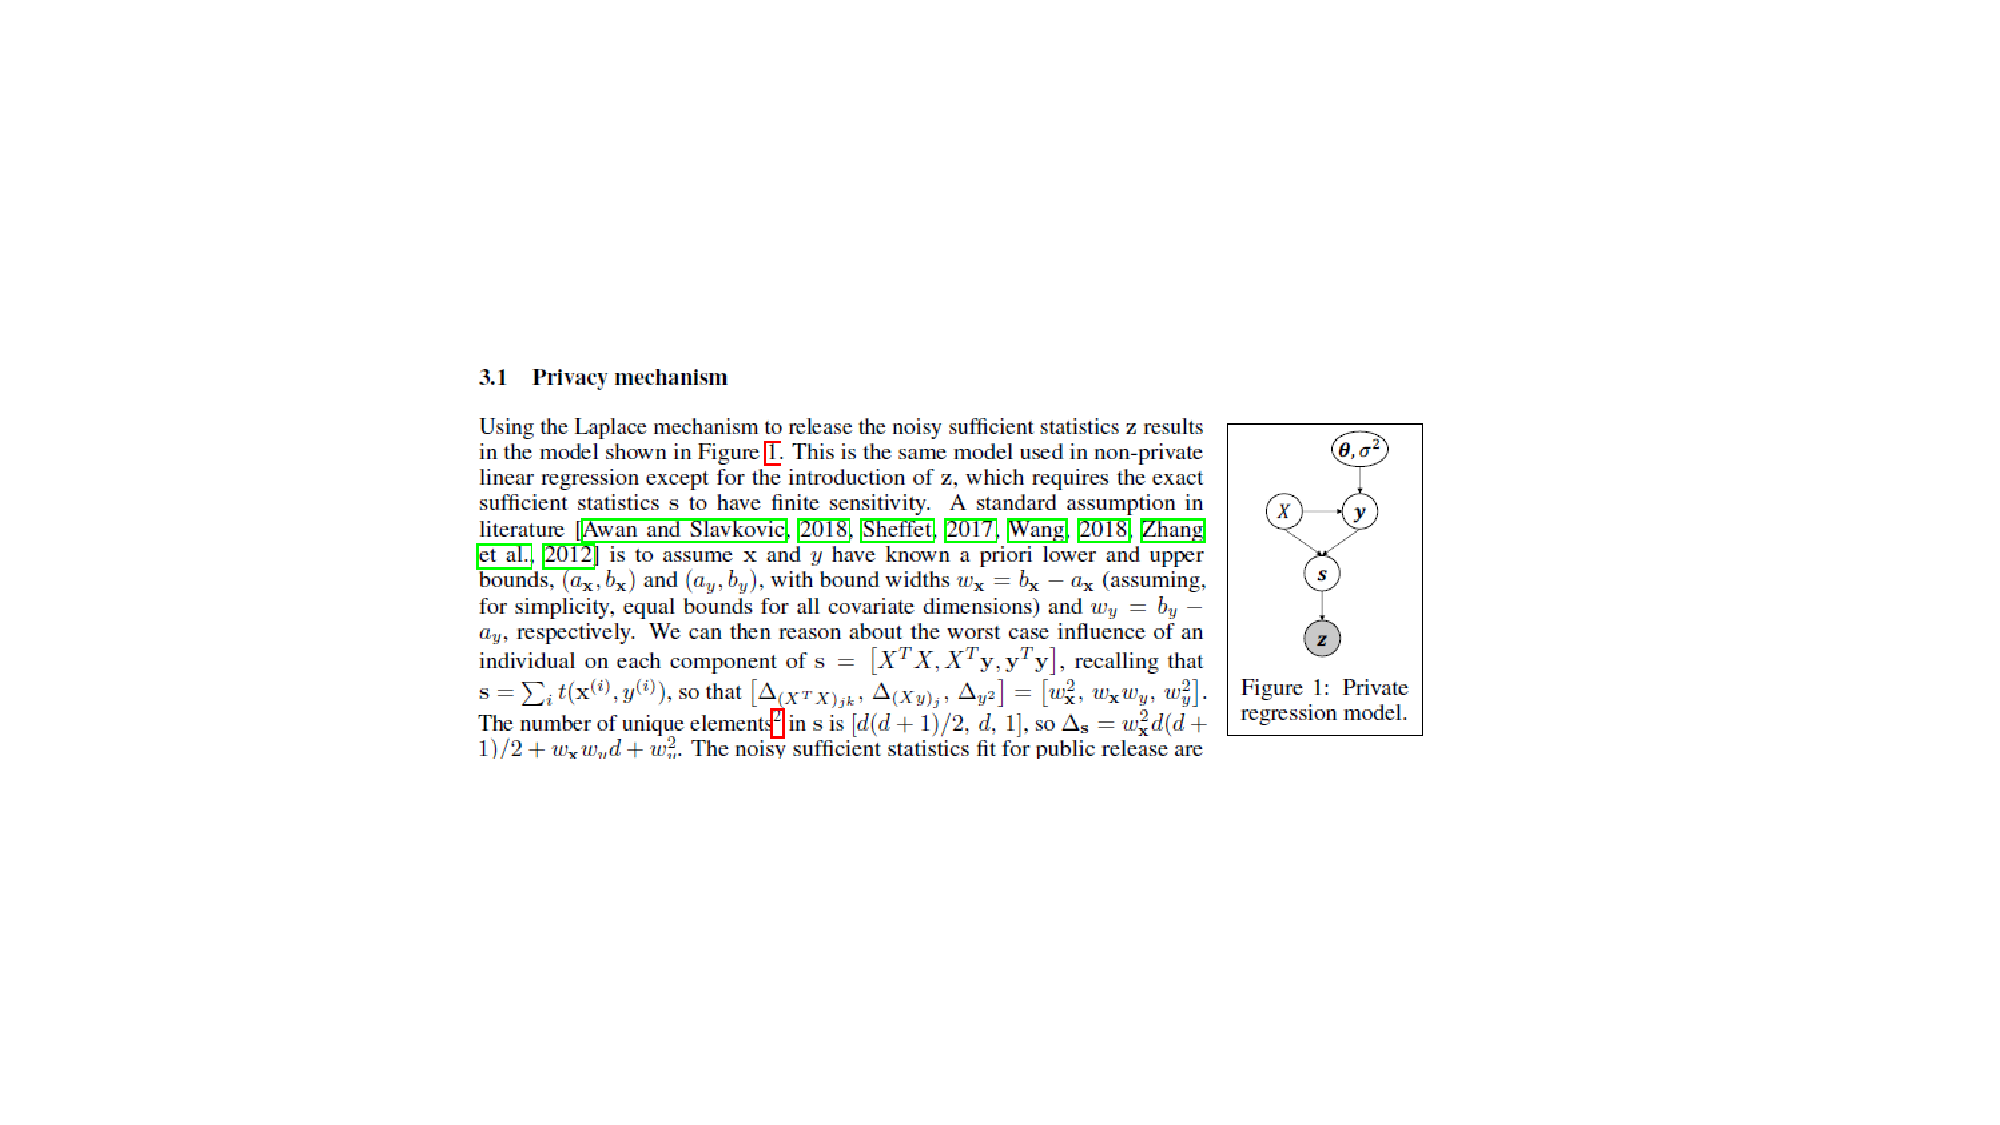
\includegraphics[trim=3in 0in 0in 2in,width=1.5\textwidth]{testcut.pdf}
  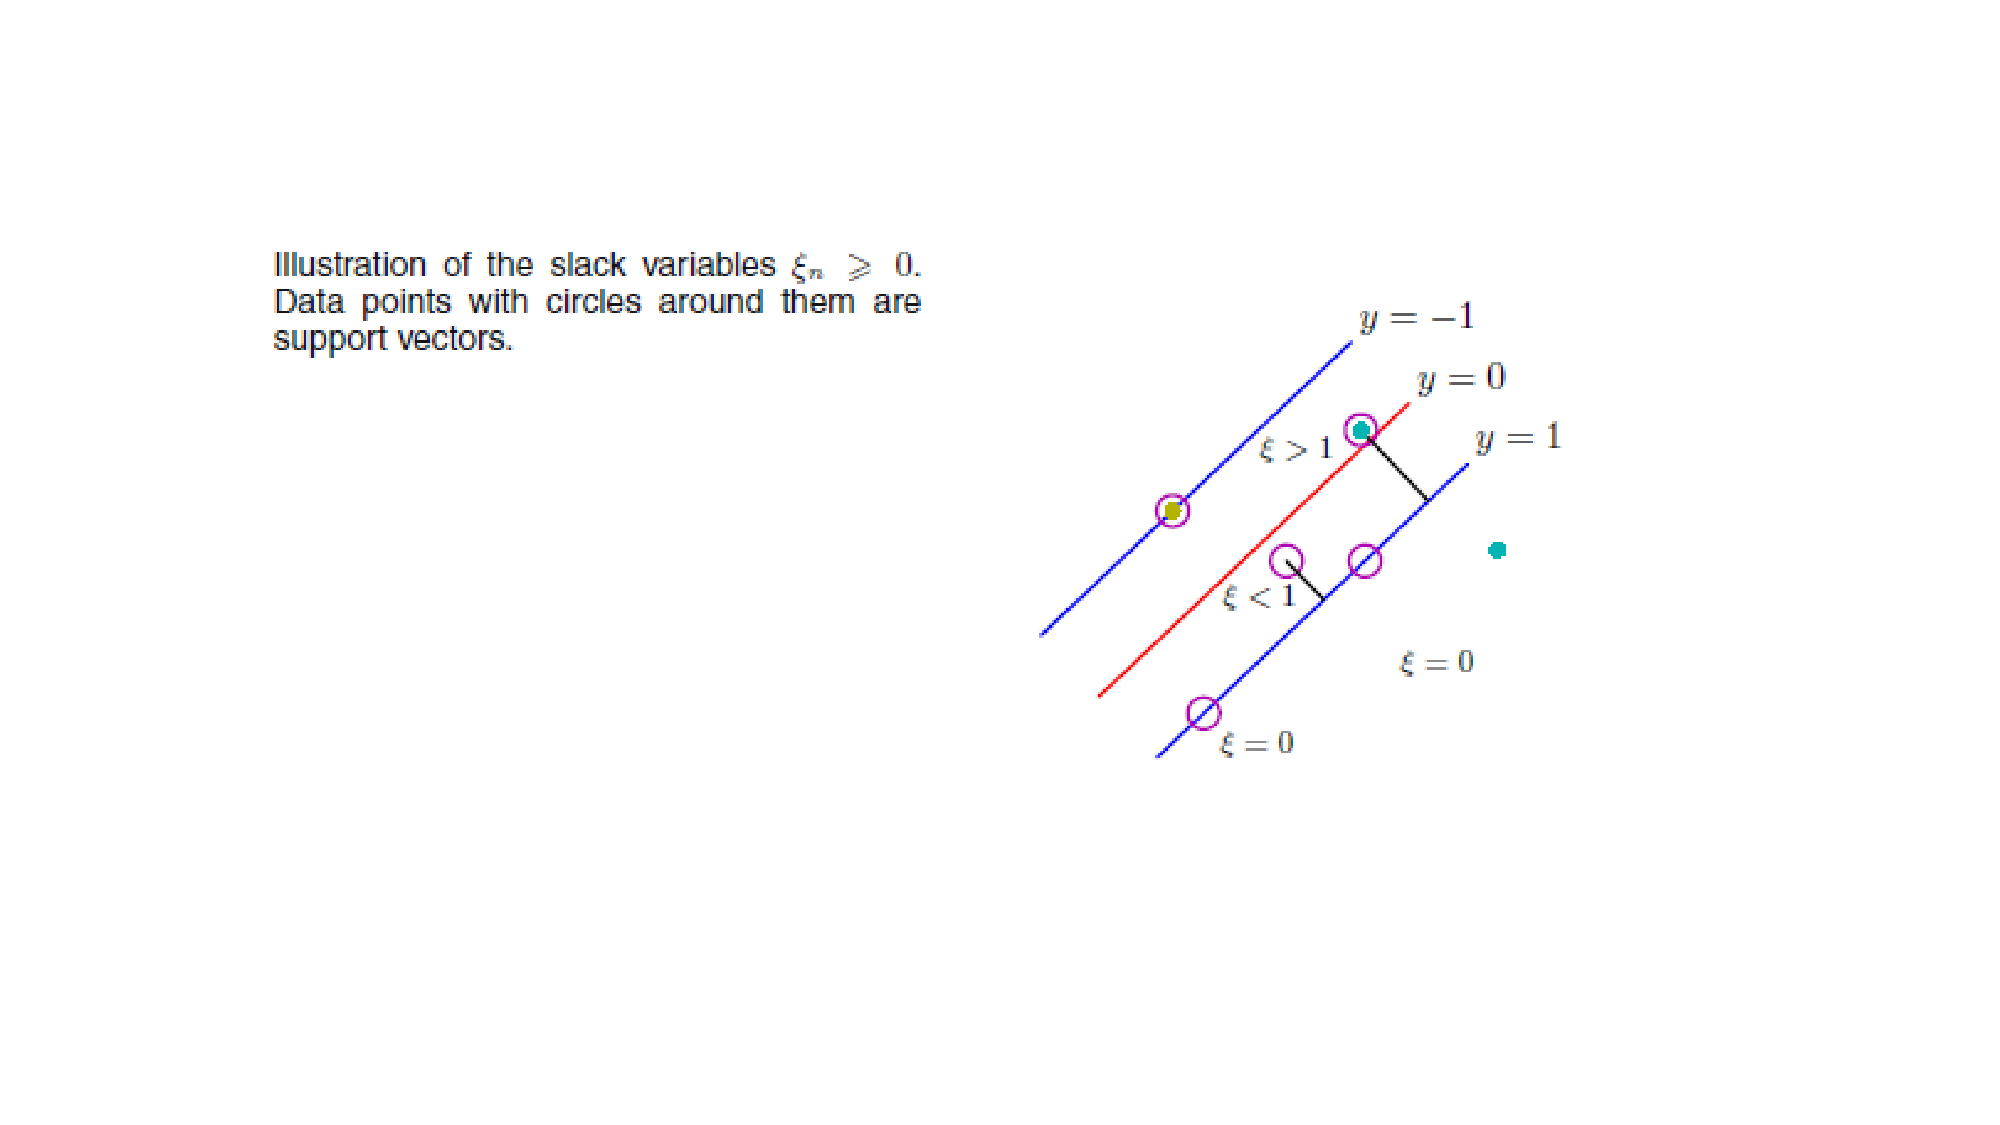
\includegraphics[trim=1.8in 0in 0in 1in,width=1.3\textwidth,clip]{../figures/zetas.pdf}

  
\end{titledslide}
%%%%%%%%%%%%%%%%%%%%%%%%%%%%%%%%%%%%%%%%%%%%%%%%%%%%%%%%%%%%%%%%%%%%%%
\begin{titledslide}{Allowing data on the wrong side of the margin}

  Earlier we had the following optimisation problem:

\begin{align}\begin{aligned}\min_ {w, b} \frac{1}{2} w^T w \\\begin{split}\textrm {subject to } & t_n (w^T \phi (x_n) + b) \geq 1\\
      \end{split}\end{aligned}\end{align}

  scikit learn actually solves \href{https://scikit-learn.org/stable/modules/svm.html\#svm-mathematical-formulation}{the following optimisation} (primal version)
  
\begin{align}\begin{aligned}\min_ {w, b, \xi} \frac{1}{2} w^T w + C \sum_{n=1}^{N} \xi_n\\\begin{split}\textrm {subject to } & t_n (w^T \phi (x_n) + b) \geq 1 - \xi_n,\\
      & \xi_n \geq 0, n=1, ..., N\end{split}\end{aligned}\end{align}


  
\end{titledslide}
%%%%%%%%%%%%%%%%%%%%%%%%%%%%%%%%%%%%%%%%%%%%%%%%%%%%%%%%%%%%%%%%%%%%%%
\begin{titledslide}{$C$ as regularisation}

\begin{align}\begin{aligned}\min_ {w, b, \xi} \frac{1}{2} w^T w + C \sum_{n=1}^{N} \xi_n\\\begin{split}\textrm {subject to } & t_n (w^T \phi (x_n) + b) \geq 1 - \xi_n,\\
      & \xi_n \geq 0, n=1, ..., N\end{split}\end{aligned}\end{align}
\begin{itemize}
\item ``Points for which $0 < \xi \leq 1$ lie inside the margin but
  on the correct side of the decision boundary \dots ``
\item ``\dots and those data points for which $\xi_{n} > 1$ lie
  on the wrong side of the decision boundary and are misclassified''
  \cite[p.332]{bishop06:_patter_recog_machin_learn}
\item We now have a `soft margin' where being on the wrong side of the
  margin is merely penalised and $C$ is a regularisation parameter.
\item Let's look at part of the output of \href{https://scikit-learn.org/stable/auto_examples/svm/plot_rbf_parameters.html}{this Jupypter notebook} to
  understand the effect of varying the value of $C$.
\end{itemize}
  
\end{titledslide}
%%%%%%%%%%%%%%%%%%%%%%%%%%%%%%%%%%%%%%%%%%%%%%%%%%%%%%%%%%%%%%%%%%%%%
\begin{titledslide}{RBF SVM classification}

\includegraphics[width=\textwidth,height=\textheight]{../figures/rbfs.pdf}
  
\end{titledslide}
%%%%%%%%%%%%%%%%%%%%%%%%%%%%%%%%%%%%%%%%%%%%%%%%%%%%%%%%%%%%%%%%%%%%%%
\begin{titledslide}{scikit learn's decision function}

The red/blue areas in the plots on the last slide represent values of
the \emph{decision function} which is defined
\href{https://scikit-learn.org/stable/modules/svm.html\#svm-mathematical-formulation}{in
  the scikit learn documentation.}
  
  \begin{equation}
    \label{eq:decisionfunction}
\sum_{i\in SV} y_i \alpha_i K(x_i, x) + b,    
  \end{equation}

  
\end{titledslide}
%%%%%%%%%%%%%%%%%%%%%%%%%%%%%%%%%%%%%%%%%%%%%%%%%%%%%%%%%%%%%%%%%%%%%% 
\begin{titledslide}{RBF SVMs are non-parametric}

  \begin{itemize}
  \item Recall that `the' RBF kernel is: $\exp(-\gamma \|x-x'\|^2)$
  \item SVMs with RBF kernels are \emph{non-parametric}. The number of
    support vectors (and thus dual parameters) depends on the data\\
    (and value of $\gamma$).
  \end{itemize}

  \vspace{1cm}
  
  \begin{quote}
    Intuitively, the gamma parameter defines how far the influence of a
    single training example reaches, with low values meaning `far' and
    high values meaning `close'. The gamma parameters can be seen as the
    inverse of the radius of influence of samples selected by the model
    as support vectors. (scikit-learn docs)
  \end{quote}

% \begin{quote}
%   The C parameter trades off correct classification of training
%   examples against maximization of the decision function's margin. For
%   larger values of C, a smaller margin will be accepted if the
%   decision function is better at classifying all training points
%   correctly. A lower C will encourage a larger margin, therefore a
%   simpler decision function, at the cost of training accuracy. In
%   other words C behaves as a regularization parameter in the SVM.
% \end{quote}

\end{titledslide}
%%%%%%%%%%%%%%%%%%%%%%%%%%%%%%%%%%%%%%%%%%%%%%%%%%%%%%%%%%%%%%%%%%%%%%
\begin{titledslide}{Multiclass classification}

  \begin{itemize}
  \item SVMs are fundamentally two class classifiers.
  \item If there are $k$ classes, approaches include:
    \begin{description}
    \item[one-versus-one] where we train $k(k-1)/2$ SVM classifiers to
      distinguish between each pair of classes (and then take a `vote'
      for the predicted class)
    \item[one-versus-the-rest] where we train $k$ SVM classifiers to
      distinguish between each class and all other classes.
    \end{description}
  \item In scikit-learn, SVC and NuSVC go for one-versus-one and
    LinearSVC does one-versus-the-rest.
  \item \href{https://scikit-learn.org/stable/auto_examples/svm/plot_iris_svc.html}{This Jupyter notebook} provides an example of
    multi-class learning with various choices of kernel.
  \end{itemize}
  
\end{titledslide}
%%%%%%%%%%%%%%%%%%%%%%%%%%%%%%%%%%%%%%%%%%%%%%%%%%%%%%%%%%%%%%%%%%%%%%
\begin{titledslide}{Reading}

  \begin{itemize}
  \item Bishop \S6.1.
  \item Bishop \S7.1 (can skip \S7.1.2). 
  \item Murphy \S17.3 up to \S17.3.8 (skip \S17.3.5 and \S17.3.6)
  \end{itemize}
  
  
\end{titledslide}
%%%%%%%%%%%%%%%%%%%%%%%%%%%%%%%%%%%%%%%%%%%%%%%%%%%%%%%%%%%%%%%%%%%%%%
\begin{titledslide}{Problems and quizzes}

  \begin{itemize}
  \item No problems
  \item Quizzes:
    \begin{itemize}
    \item Week~3: Intro to Kernels
    \item Week~3: SVMs
    \item Week~3: SVMs in Practice
    \end{itemize}
  \end{itemize}
  
\end{titledslide}

\bibliographystyle{alpha}
\bibliography{../ml.bib}


\end{document}



